\documentclass[a4j, fleqn, 12pt]{jsreport}
\usepackage{bm}
\usepackage[dvipdfmx]{graphicx}
\usepackage{listings}
\usepackage{fancyhdr}
\usepackage{amsmath}
\usepackage{bm}
\usepackage{setspace}
\usepackage{url}
\usepackage{multirow}
\usepackage{multicol}
\usepackage{float}
\usepackage{pifont}
\usepackage[hang,small,bf]{caption}
\usepackage[subrefformat=parens]{subcaption}

\usepackage{STY/h25-GT}
\usepackage{STY/arydshln}

\usepackage{enumerate}
\def\circledenumerate#1{\textcircled{\scriptsize #1}}
\def\MARU#1{\leavevmode \setbox0\hbox{$\bigcirc$}
\copy0\kern-\wd0 \hbox to\wd0{\hfil{#1}\hfil}}

\usepackage{caption}
\captionsetup{font=small, labelfont=small}
\captionsetup{compatibility=false}
\captionsetup[subfigure]{labelformat=simple}
\renewcommand{\thesubfigure}{(\alph{subfigure})}

\lstset{
    basicstyle={\ttfamily},
    identifierstyle={\small},
    commentstyle={\smallitshape},
    keywordstyle={\small\bfseries},
    ndkeywordstyle={\small},
    stringstyle={\small\ttfamily},
    frame={tb},
    breaklines=true,
    columns=[l]{fullflexible},
    numbers=left,
    xrightmargin=0zw,
    xleftmargin=3zw,
    numberstyle={\scriptsize},
    stepnumber=1,
    numbersep=1zw,
    lineskip=-0.5ex,
    keepspaces=true,
    language=c
}
\renewcommand{\lstlistingname}{リスト}
\makeatletter
\newcommand{\figcaption}[1]{\def\@captype{figure}\caption{#1}}
\newcommand{\tblcaption}[1]{\def\@captype{table}\caption{#1}}
\makeatother

\renewcommand{\chaptermark}[1]{\markboth{#1}{}}
\renewcommand{\sectionmark}[1]{\markright{#1}{}}

\reportname{令和5年度電子制御工学科卒業論文}
\reporttitle{単一視点による\\人物の全身運動の三次元計測について}
\reportdate{2024/02/27}
\autheraff{
長岡工業高等専門学校\\
電子制御工学科\\
視覚情報処理研究室\\
(指導教員    高橋 章教授)
}
\reportauther{本間 三暉}
\pagestyle{fancy}
\rhead{\thesection\, \rightmark}
\lhead{第\ \thechapter\ 章\, \leftmark}
\rfoot{視覚情報処理研究室}

\begin{document}
\pagenumbering{roman}
\maketitle
\tableofcontents
\cleardoublepage
\pagenumbering{arabic}

\chapter{はじめに}
人の動きなどのノンバーバルな情報をコミュニケーションに用いたり,技術の継承や伝統芸能のディジタルアーカイブに利用したりするために,
カメラの二次元画像から三次元の骨格情報を推測する技術が求められている.
本研究室では柔道の三次元の動きを複数視点の動画から推測する研究\cite{turugi}が行われた.
しかし,この方法では複数台のカメラを設置し,キャリブレーションを行うため,十分な広さを持つ測定空間が必要である.
また,近年技術開発が進んだことにより,物体までの奥行きの情報(デプス)を取得できるカメラが市販されたり,
機械学習によって単眼カメラから深度推定を行う方法\cite{depth}が提案されたりしている.

そこで本研究では機械学習を活用して一台の入力装置で三次元骨格推定を行う手法として,
RGB画像を入力する方法とRGB画像に加えてデプス情報を入力する方法を実装する.
さらに慣性式モーションキャプチャデバイスによる計測結果と比較するための座標系及び時間のキャリブレーション方法を検討する.

\chapter{研究内容・方法}
人の動作の三次元骨格推定を行う方法として,画像処理による方法やモーションセンサによる方法がある.それぞれの方法について簡単にまとめたものを表\ref{3D_1}に示す.
画像処理による三次元骨格推定は撮影するカメラに,色情報を記録できる一般的なRGBカメラを用いる方法と,
物体のデプスも取得可能なRGBDカメラを用いる方法がある(\ref{3Dskeleton}節).

モーションセンサによる方法は,光学式や慣性式などがある.
光学式は体表面にマーカーを取り付けそのマーカーを複数台のカメラで取り込むことで骨格を高精度に推定できるが広い計測空間が必要になる.
慣性式は加速度,角速度,方位を測定できるセンサを体表面の指定箇所に取り付けることで骨格を推定する(\ref{motion}節).

%%%あまりにも急展開

本研究では,市販の入力デバイスを使用する3つの推定方法を実装して性能を比較評価する.
\begin{table}[b!]
  \centering
  \caption{動作を計測する方法の種類と特徴}
  \begin{tabular}{c|cc|cc}
    \hline
<<<<<<< HEAD
                  & \multicolumn{2}{c|}{\small{カメラ}}       & \multicolumn{2}{c}{\small{モーションセンサ}}                                                   \\ \cline{2-5}
                  & \multicolumn{1}{c|}{\small{RGB}}       & \small{RGBD}                         & \multicolumn{1}{c|c}{\small{光学式}} & \small{慣性式} \\ \hline
    \small{センサ装着} & \multicolumn{1}{c|}{\small{不要}}        & \small{不要}                           & \multicolumn{1}{c|}{\small{必要}}   & \small{必要}  \\
    \small{外から撮影} & \multicolumn{1}{c|}{\small{必要}}        & \small{必要}                           & \multicolumn{1}{c|}{\small{必要}}   & \small{不要}  \\
    \small{必要台数}  & \multicolumn{1}{c|}{\small{1$\sim$数台}} & \small{1台}                           & \multicolumn{1}{c|}{\small{複数}}   & \small{0}   \\ \hline
=======
                  & \multicolumn{2}{c|}{\small{カメラ}}       & \multicolumn{2}{c}{\small{モーションセンサ}}                                                  \\ \cline{2-5}
                  & \multicolumn{1}{c|}{\small{RGB}}       & \small{RGBD}                         & \multicolumn{1}{c|}{\small{光学式}} & \small{慣性式} \\ \hline
    \small{センサ装着} & \multicolumn{1}{c|}{\small{不要}}        & \small{不要}                           & \multicolumn{1}{c|}{\small{必要}}  & \small{必要}  \\
    \small{外から撮影} & \multicolumn{1}{c|}{\small{必要}}        & \small{必要}                           & \multicolumn{1}{c|}{\small{必要}}  & \small{不要}  \\
    \small{必要台数}  & \multicolumn{1}{c|}{\small{1$\sim$数台}} & \small{1台}                           & \multicolumn{1}{c|}{\small{複数}}  & \small{0}   \\ \hline
>>>>>>> 618ecf307d12c9a6695c09af37e2dd7af997384b
  \end{tabular}
  \label{3D_1}
\end{table}
\section{慣性式モーションキャプチャの三次元骨格推定}\label{motion}
慣性式モーションキャプチャデバイスとしてmocopi\cite{mocopi}を用いる.
mocopiのセンサは3つの自由度を持つ角度センサと加速度センサを搭載している.
両手,両足,頭,腰の計6ヶ所にセンサを装着してリアルタイムに三次元計測を行うことができる.
センサを装着しない肘や膝などの関節部を直接測定することはできないが,
機械学習を用いることでp.\pageref{mocopi}の図\ref{mocopi}に示すような27個の関節位置を推定している.

mocopiは専用のスマホアプリでモーションを収録することでBVHファイル(付録\ref{BVH_file}を参照)での書き出しが可能である.
この時mocopiのモーションデータのフレームレートは30,50,60\,fpsから選ぶことが可能である.
書き出したBVHファイルはホストとなるスマホの機種により保存されるフォルダが異なり,iphoneの場合mocopiフォルダのMotionData配下,Androidスマホの場合ユーザーが初回保存時に指定したフォルダ配下に保存される.

本研究ではホストとなるスマホにiPhone\,SE(第2世代)とGoogle\,Pixel\,8を用いた.
しかし,Google\,Pixel\,8ではモーションセンサとの接続が不安定となってしまうため,測定にはiPhone\,SE(第2世代)をホストとした.
また,モーションデータのフレームレートは60\,fpsとした.

\section{画像処理による三次元骨格推定}\label{3Dskeleton}
画像処理を用いて三次元骨格推定をしている様子をp.\pageref{image_3D}の図\ref{image_3D}に示す.
本研究では画像入力装置としてRGBDカメラであるIntel RealSense D415(以下RealSense)を使用する.
RealSenseのスペックを付録\ref{D415}に示す.
% \begin{table}[t]
%   \centering
%   \caption{Intel RealSense D415のスペック}
%   \begin{tabular}{l|l}
%     \hline
%     {\small 使用環境}                                  & {\small 屋内/屋外}                                     \\
%     {\small 深度技術}                                  & {\small Active IR stereo(ローリングシャッター)}              \\
%     {\small 主要Intel RealSenseコンポーネント}              & {\small Intel RealSense Vision Processor D4}       \\
%                                                    & {\small Intel RealSense module D410}               \\
%     {\small 深度センサ視野角(水平 $\times$ 垂直 $\times$ 斜め)}  & {\small 69.4°$\times$ 42.5°$\times$ 77°(±3°)}      \\
%     {\small 出力解像度(DepthStream)}                    & {\small 最大1280 $\times$ 720}                       \\
%     {\small 出力フレームレート(DepthStream) }               & {\small 最大90\,fps}                                 \\
%     {\small 最小深度距離(Min-Z)}                         & {\small 0.3\,m}                                    \\
%     {\small シャッタータイプ}                              & {\small ローリングシャッター}                                \\
%     {\small 最大レンジ}                                 & {\small 約10 m(較正,背景,照度状況による)}                      \\
%     {\small 解像度およびフレームレート(RGBセンサ)}                 & {\small 1920 $\times$ 1080@30\,fps }               \\
%     {\small RGBセンサ視野角(水平 $\times$ 垂直 $\times$ 斜め)} & {\small 69.4° $\times$ 42.5° $\times$ 77°(±3°)}    \\
%     {\small 本体寸法(長さ $\times$ 奥行き $\times$ 高さ)}     & {\small 99 mm $\times$ 20 mm $\times$ 23 mm}       \\
%     {\small コネクタ}                                  & {\small USB 3.0 Type-C}                            \\
%     {\small 取付機構}                                  & {\small 1 $\times$ 1/4-20 UNCネジ穴、2 $\times$ M3ネジ穴} \\
%     {\small 測定原理}                                  & {\small アクティブステレオ法}                                \\\hline%(付録\ref{active})
%   \end{tabular}
%   \label{D415}
% \end{table}

RealSenseはカメラから物体までの距離を図る方法として,RealSense内部のプロジェクタとカメラを用いてアクティブステレオ法を行っている.
アクティブステレオ法とは,プロジェクタから投影するパターンの画像と,カメラの画像との間でマッチングを行うことで距離を測定する方式である.
投影するパターンは不可視の赤外線を利用している.

RealSenseから手に入れたRGBD画像からRGB画像を取り出し,RGB画像とRGBD画像それぞれを入力とする.
2種類の入力画像からそれぞれ画像処理を用いて骨格推定をする方法として2つの方法を実装する.

1つ目はカラー画像を入力としてGoogleが提供するオープンソースの機械学習ライブラリMediaPipe Pose\cite{mediapipe}を用いることで図\ref{RGB}に示す33個の関節の三次元骨格情報を取得する方法である.
MediaPipe Poseは三次元の骨格情報と二次元画像を関連付けたデータを元に機械学習をすることで,二次元画像から三次元の関節の位置情報を推定することを可能にしている.
実装した様子をp.\pageref{RGB_uu}の図\ref{RGB_uu}に示す.

2つ目はカラー画像とデプス情報を入力として3DiVi Incが提供するライブラリNuitrack\cite{nuitrack}を用いることで図\ref{RGBD}に示す19個の関節の三次元骨格情報を取得する方法である.
Nuitrackは機械学習と3DiVi社独自のアルゴリズムによって,RGBD画像から三次元の関節の位置情報を推定できる.
実装した様子をp.\pageref{RGBD_uu}の図\ref{RGBD_uu}に示す.

\begin{figure}[t]
  \centering
  \begin{minipage}[]{0.45\hsize}
    \centering
    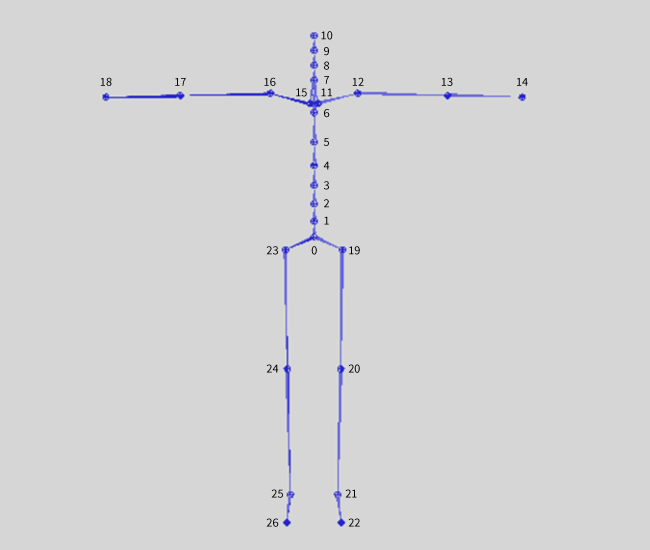
\includegraphics[width=6cm]{img/TechSpec_02.png}
    \subcaption{mocopiで取得できる関節位置}
    \label{mocopi}
  \end{minipage}
  \begin{minipage}[]{0.45\hsize}
    \centering
    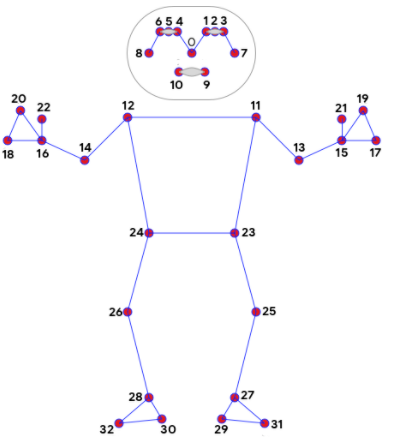
\includegraphics[width=6cm]{img/media.png}
    \subcaption{MediaPipe Poseで取得できる関節位置}
    \label{RGB}
  \end{minipage}\\
  \begin{minipage}[]{0.45\hsize}
    \centering
    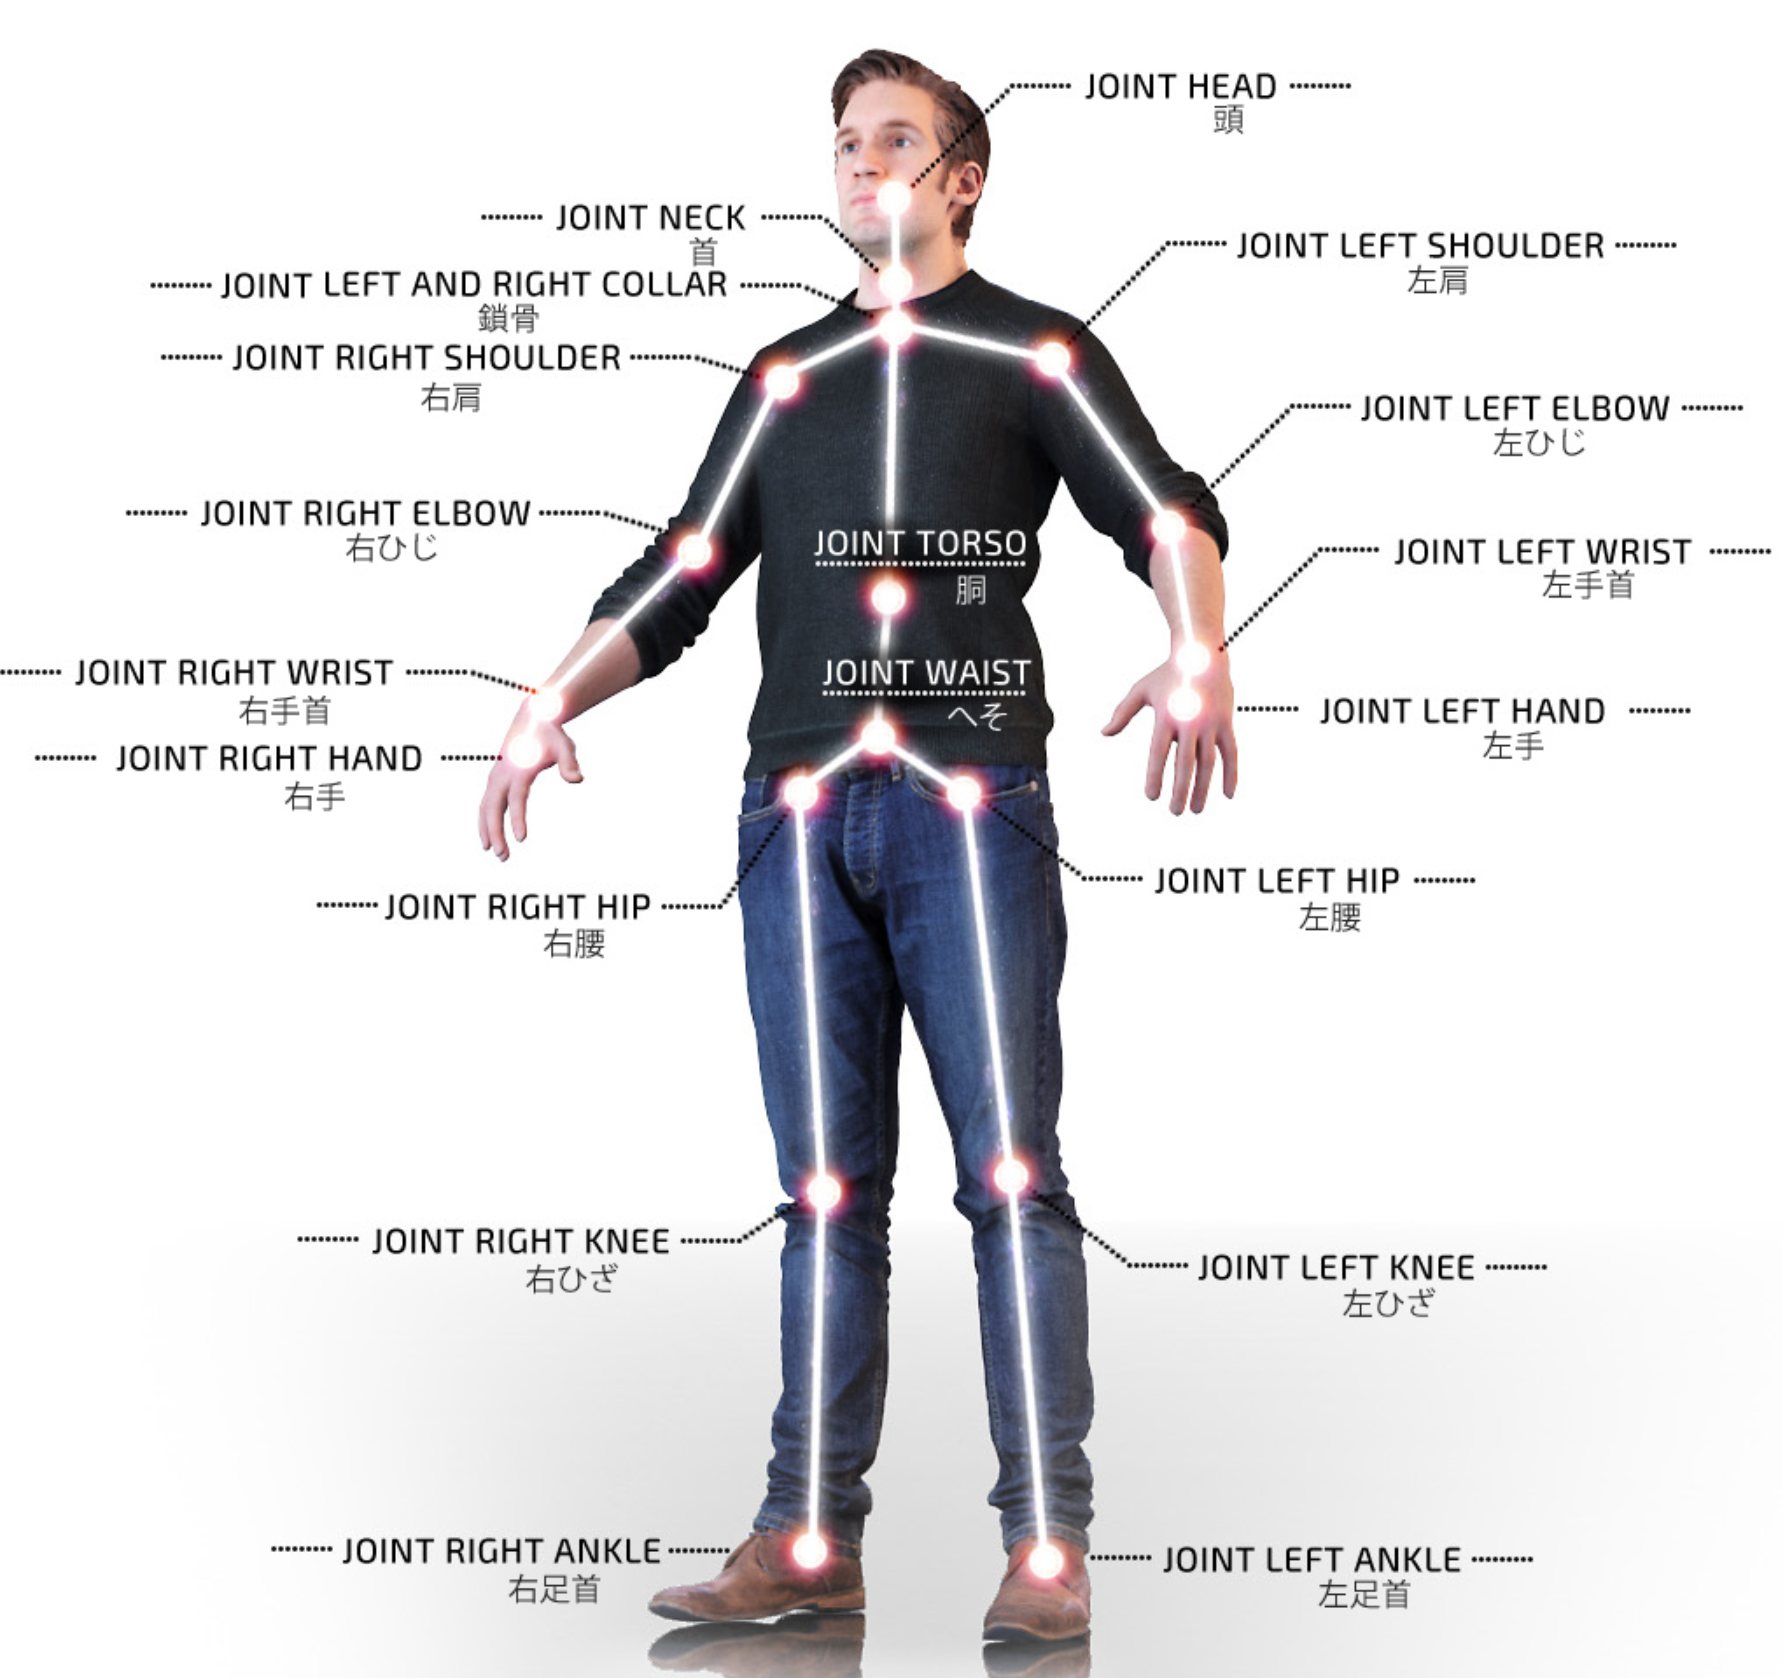
\includegraphics[width=6cm]{img/nuitrack.png}
    \subcaption{Nuitrackで取得できる関節位置}
    \label{RGBD}
  \end{minipage}
  \caption{各ライブラリで取得できる骨格の関節位置}
  \label{sokutei}
\end{figure}

\begin{figure}[t]
  \centering
  \begin{minipage}[]{0.45\hsize}
    \centering
    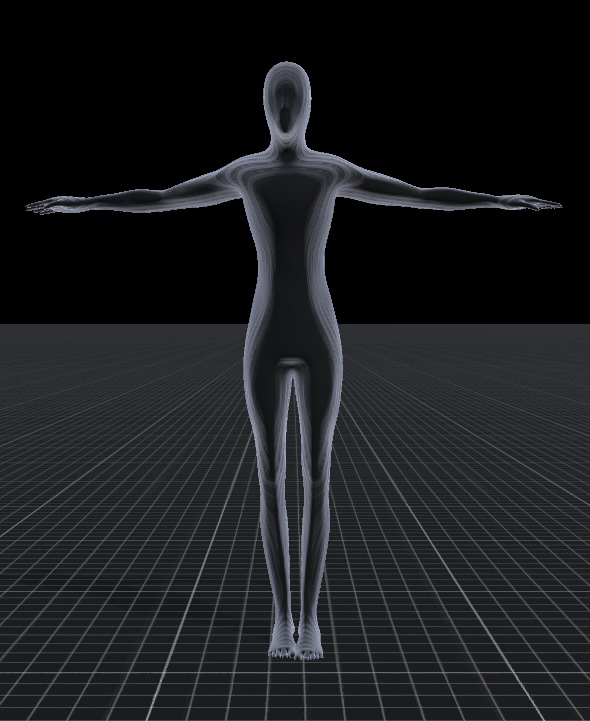
\includegraphics[width=5cm]{img/mocopi_uu.png}
    \subcaption{mocopiで取得できる関節位置}
    \label{mocopi_uu}
  \end{minipage}
  \begin{minipage}[]{0.45\hsize}
    \centering
    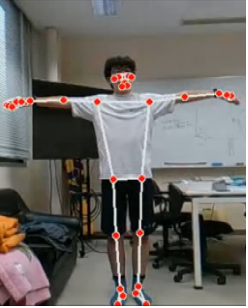
\includegraphics[width=5cm]{img/media_uu.png}
    \subcaption{MediaPipe Poseで骨格推定した様子}
    \label{RGB_uu}
  \end{minipage}\\
  \begin{minipage}[]{0.45\hsize}
    \centering
    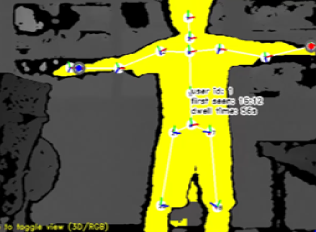
\includegraphics[width=7cm]{img/nuitrack_uu.png}
    \subcaption{Nuitrackで骨格推定した様子}
    \label{RGBD_uu}
  \end{minipage}
  \caption{各ライブラリで骨格推定した様子}
  \label{sokutei_uu}
\end{figure}
\begin{figure}[b]
  \centering
  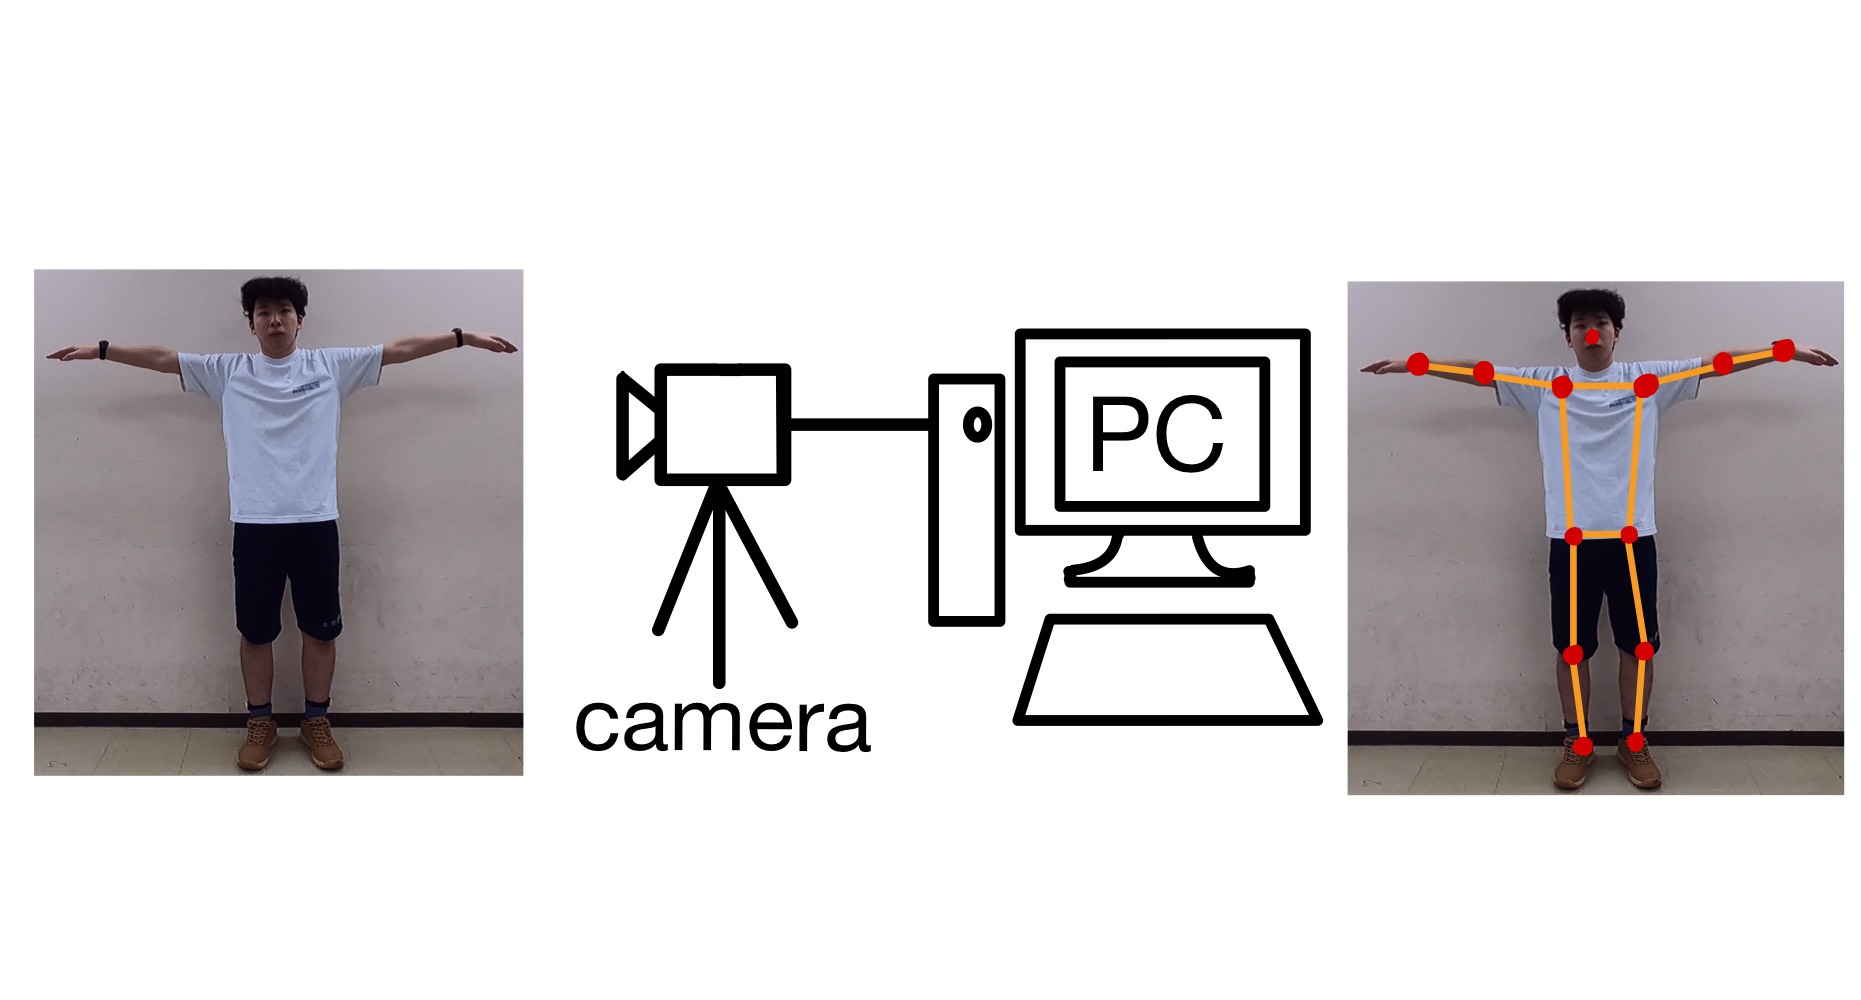
\includegraphics[width=10cm]{img/image_3D.png}
  \caption{画像処理による骨格推定の様子}
  \label{image_3D}
\end{figure}

% \newpage
\clearpage
\section{キャリブレーション}\label{kyari}
推定方法によって骨格座標のスケールや基準となる座標系が違うので,定量的に比較評価するためには座標系を統一する必要がある.
そこで計測開始時に,両腕を水平に上げるポーズを取ることにする.水平に上げた両手首の距離を元にスケールを合わせる.
また,へその位置を原点として,頭に向かう方向をy軸,右手から左手に向かう方向をx軸,これらに軸の直交する方向をz軸と定める.

動作の比較を行うには同期を取る必要があるが,画像処理による方法とmocopiを用いる方法では互いの同期計測ができない.
そこで座標系を合わせるポーズの後で両手を伸ばしたまま胸の前で合わせるポーズをする.
手が合わさっている時,両手首が最接近するので,各骨格情報の両手首の座標が最も近づいたフレームを時刻の基準と定める.

\chapter{研究結果}
\section{実験方法}
一名の被験者(男子学生)が\ref{kyari}節に示す骨格情報のキャリブレーションに必要なポーズを行い,正しくキャリブレーションできているか評価する.
座標軸のキャリブレーションのポーズである手を広げた状態から,時間軸の基準となる両手が最接近した状態になるまでは170フレームで行われている.
手を広げたポーズを取ったとき,へそを原点,体の中心から右手首までの距離を1としたx-z平面で表す.
\section{解析結果}
Nuitrackによる方法では関節の位置座標を取得することが困難であったため,mocopiとMediaPipe Poseによる方法で取得した骨格座標情報を示す.
mocopiにより取得した右手首の骨格座標情報を図\ref{fig:1_mocopi},MediaPipe Poseにより取得した両手首の骨格座標情報を図\ref{fig:1_media}に示す.


\begin{figure}[h]
  \centering
  \begin{minipage}{10cm}
    \centering
    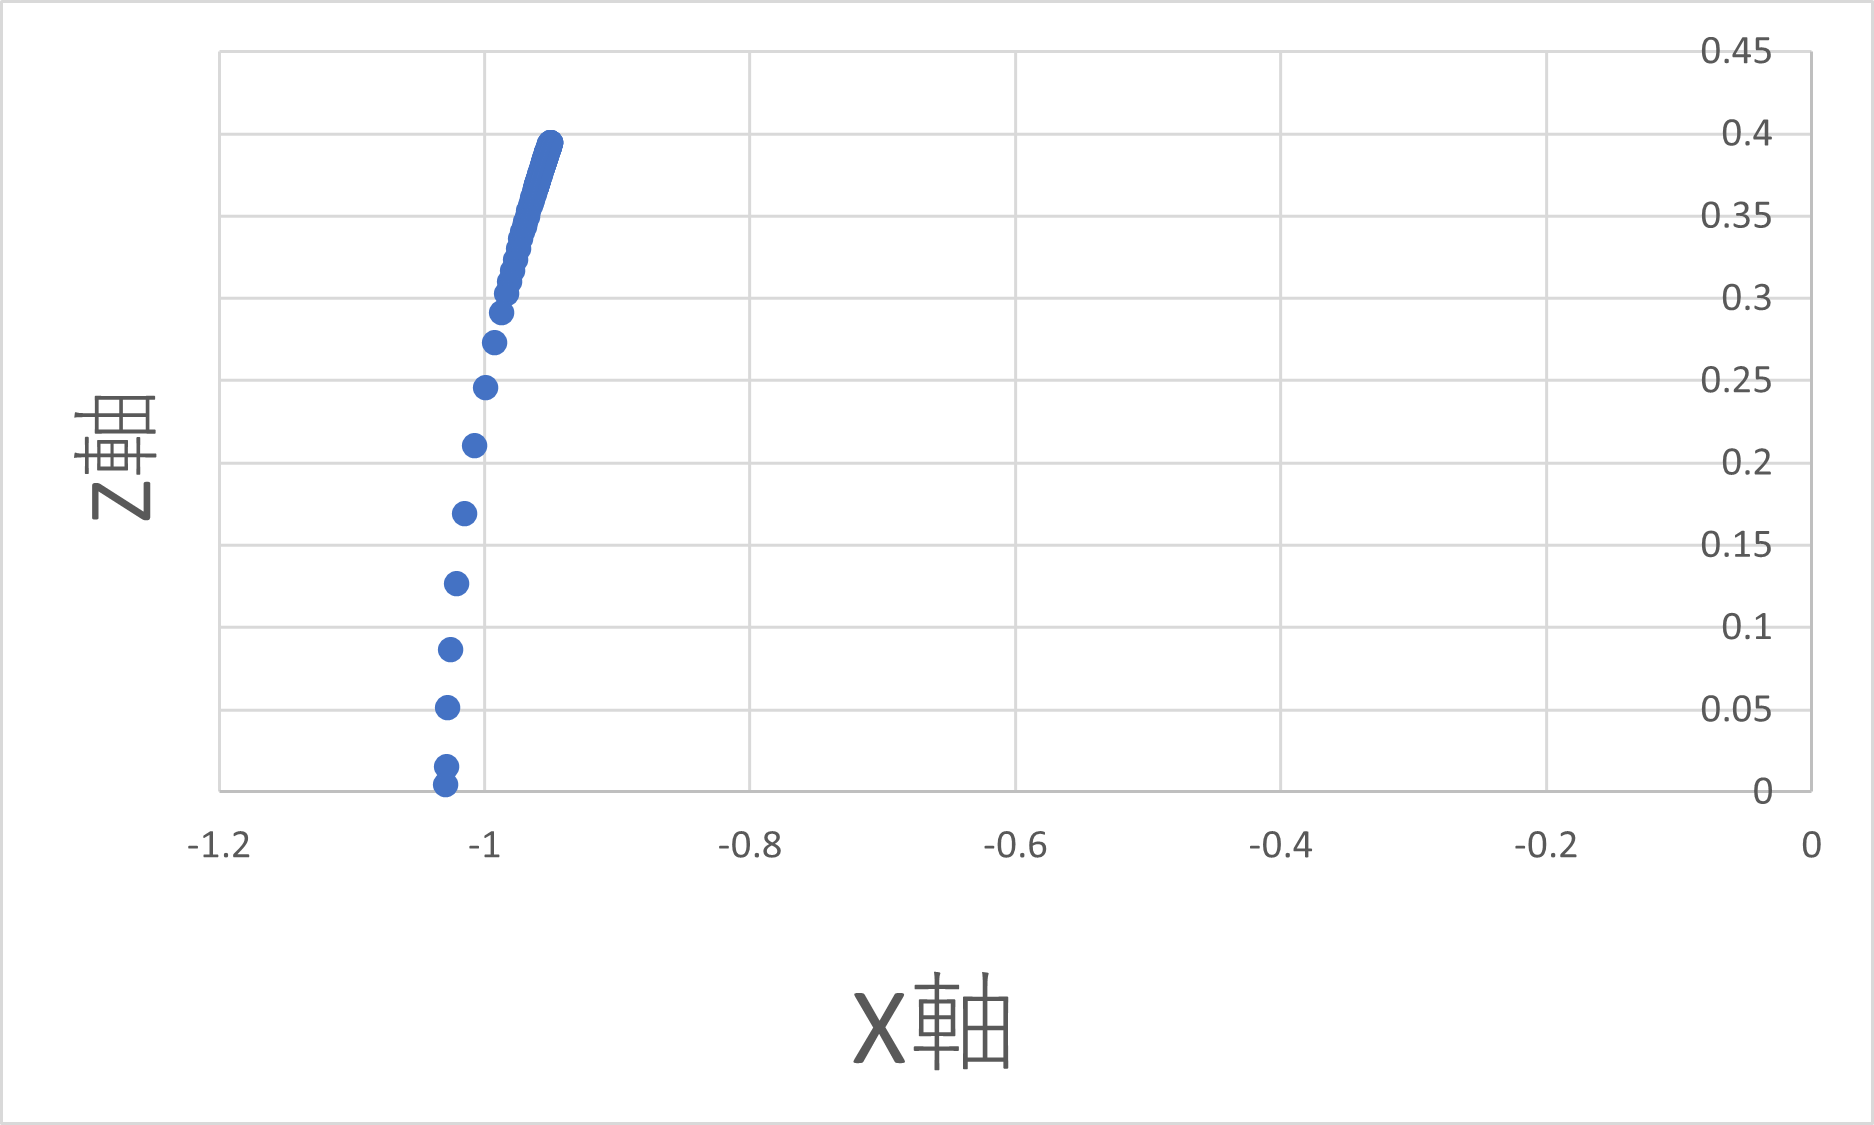
\includegraphics[width=10cm]{img/1_mocopi.png}
    \caption{mocopiで得た両手首の位置情報}
    \label{fig:1_mocopi}
  \end{minipage}\\
  \begin{minipage}{10cm}
    \centering
    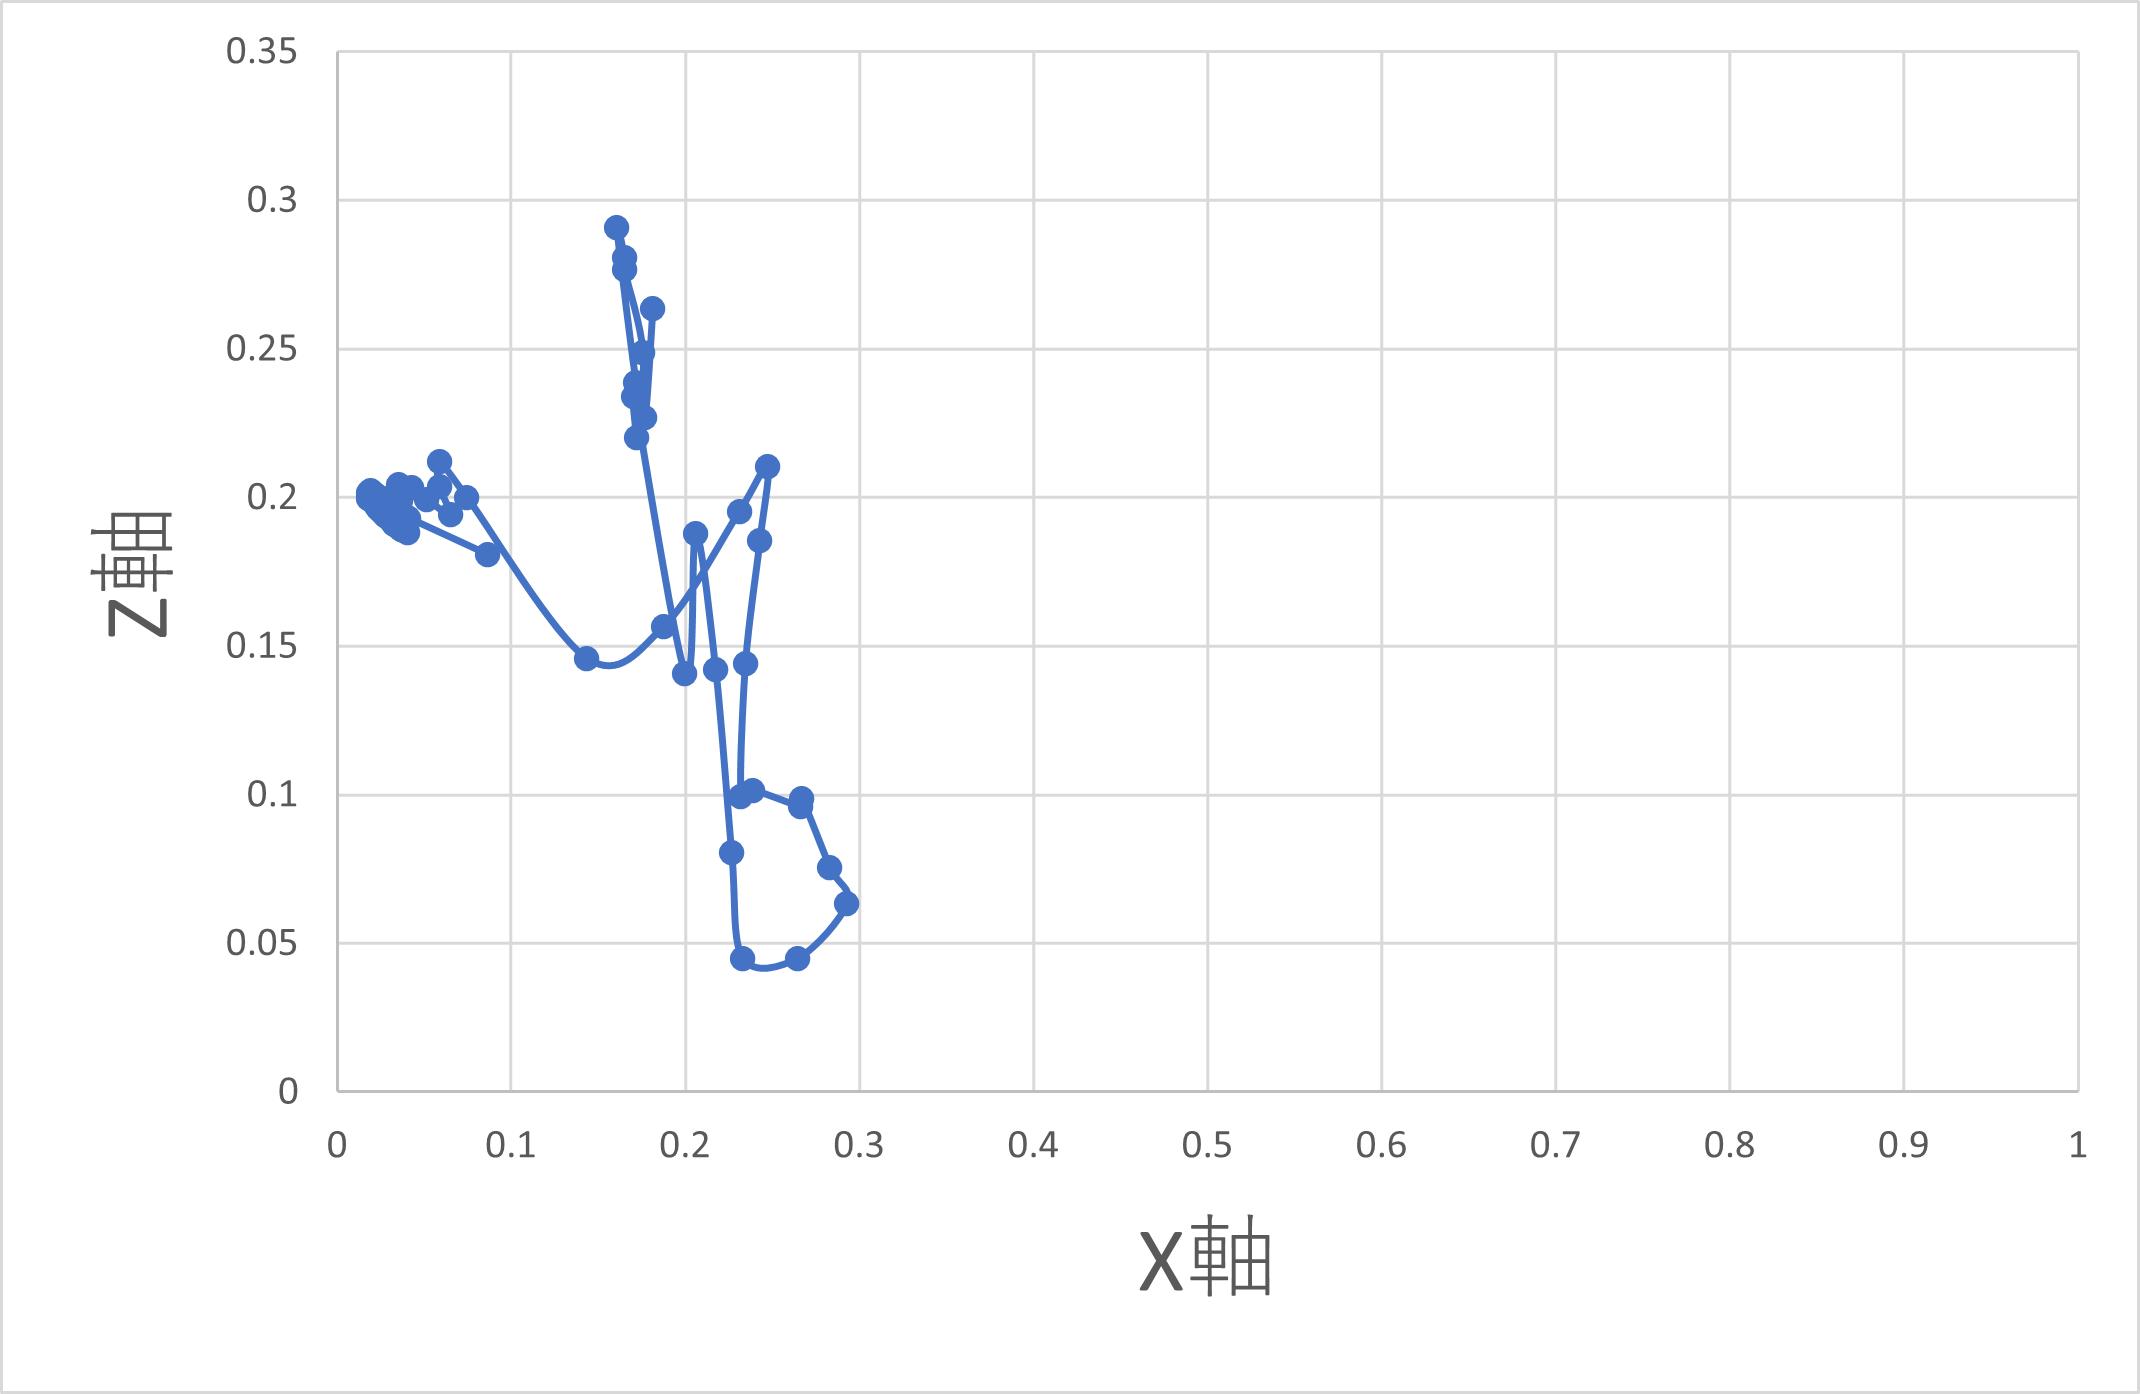
\includegraphics[width=10cm]{img/1_media.png}
    \caption{MediaPepe Poseで得た両手首の位置情報}
    \label{fig:1_media}
  \end{minipage}
\end{figure}
今回行ったキャリブレーションのポーズでは,カメラから見てへそより前に両手首があるので,z軸方向の値が負になることはありえない.
また,へその前まで腕を持ってきているので,正しく計測できていれば両手首の座標をx-z平面に示した際の軌跡は原点を中心とした半径1の円に似た軌道を描くはずである.

mocopiは実際の骨格の三次元位置より,動作の滑らかさを優先していることがわかった.
動かした際の人間らしくない動きをなくすためではないかと考えられる.

MediaPipe Poseは多少のノイズがあるが,体に対し平行な向きはある程度正確に測定できることがわかった.
しかし,奥行き方向に歪んでいることもわかった.
\chapter{まとめ}
本研究では,キャリブレーションの方法として2つのポーズを続けて行い,3種類の手法を定量的に比較するためのキャリブレーションを試みた.
また,mocopiによる方法では各骨格の三次元位置より動作の滑らかさを優先している事がわかった.
RGBカメラによる方法では機械学習を用いて奥行き情報を取得できる方法を用いたが,慣性式モーションキャプチャデバイスで取得した骨格データよりノイズが大きくなることが確認できた.

今後の課題として,Nuitrackを用いて三次元骨格推定を行った場合の関節の位置座標を取得しキャリブレーションを行う.
また,今回実装した3種類の方法を比較した際に,それぞれどのような特徴がどのような理由で出るのか考察を行う.
mocopiの骨格データを補正する事はできないか検証を行うことなどが挙げられる.
% 今後の課題として,RGBDカメラを用いて撮影したデータから推定した座標データに対してキャリブレーションを行った場合についても.
% RGBDによる方法では現在問題の修正中であるがRGBDによる方法を用いることで.デプス情報を元に正しく測定できるのではないかと考えられる.
\section*{謝辞}
本研究におきまして,視覚情報処理研究室の高橋章教授から多大なるご指導,ご助力を賜りましたことを深く感謝するとともに,心から御礼申し上げます.
また,ご協力いただいた同研究室の各氏にも感謝します.

% \addcontentsline{toc}{chapter}{参考文献} %章立てせずに目次に追加するおまじない
% \renewcommand{\bibname}{参考文献} %これがないと,タイトルが「関連図書」になってしまう
\begin{thebibliography}{99}
  \small{
    \bibitem{turugi}{
      剱 一輝,``柔道競技の3Dアーカイブ化'',令和4年度長岡高専専攻科論文,2023.
    }
    \bibitem{depth}{
      北川リサ,伊藤貴之,``競技かるたにおける払いの動作の三次元ボーン表示による可視化'',情報処理学会第85回全国大会,
      2023,1,139 -- 140,2023.
    }
    \bibitem{mocopi}{
      SONY,``モバイルモーションキャプチャーmocopi'',\url{https://www.sony.jp/mocopi/}
    }
    \bibitem{BVH}{
      TMPSwiki,``MOCAPデータファイル'',\url{https://mukai-lab.org/content/MotionCaptureDataFile.pdf}
    }
    \bibitem{RS}{
      Intel,``Depth\,Camera\,D415'',\url{https://www.intelrealsense.com/depth-camera-d415/}
    }
    \bibitem{mediapipe}{
      Google,``MediaPipe'',\url{https://developers.google.com/mediapipe}
    }
    \bibitem{nuitrack}{
      3DiVi,``Nuitrack\,SDK'',\url{https://www.aerotap.com/nuiTrack/doc/Overview_page.html}
    }
    \bibitem{オイラー}{
      L.D.ランダウ,E.M.リフシッツ,``力学'',pp.138--139
    }
  }
\end{thebibliography}
\bibliography{bibtexファイル名} %bibtexファイルの読み込み
\bibliographystyle{junsrt} %本文に\cite{}を入れることで,参考文献表示

\appendix
\chapter{mocopiから出力されるBVHファイルの構造}\label{BVH_file}
BVHファイルはモーションキャプチャデータファイルフォーマットである.
BVHファイルの特徴を以下にまとめる\cite{BVH}.
\begin{itemize}
  \item テキスト形式で記述
  \item 右手座標系で,xyz各軸の扱い(どの軸が鉛直方向に対応するか等)はファイルの仕様としての指定はない
  \item 関節ノードに関する情報を記述
  \item 関節回転はオイラー角形式(付録\ref{Euler}を参照)で記述
  \item 位置の単位はcm,回転角度の単位はdegree
  \item スケルトン階層を表すHIERARCHYと,動作データを表すMOTIONの二つから構成
\end{itemize}
mocopiから出力されたBVHファイルは,右手座標系でY軸が座標系内の鉛直方向としている.
mocopiで計測したモーションデータの出力ファイルであるBVHファイルをリスト\ref{BVH}に示す.

まず,HIERARCHYのキーワードで始まる部分でスケルトンの構造を定義している.
各関節のボーンの長さと初期方向,関節の親子関係,関節自由度の情報が記述されている.

ROOTは階層構造の始点となり,OFFSET,CHANNELSを要素に持ち,必ず1つ以上のJOINTもしくはEndを持つ.
JOINTはOFFSET,CHANNELSを要素に持ち,必ず1つ以上のJOINTもしくはEndを持つ.
Endは階層構造の末尾となる特殊なJOINTである.
OFFSETは親ノードから子ノードへの三次元の相対的な初期位置で,ROOTの場合座標系内の絶対的な初期位置である.
CHANNELは,関節自由度に続き,位置の自由度 (Xposition,Yposition,Zposition),
回転の自由度(Xrotation,Yrotation,Zrotation)を,ROOTから子ノードに向かう順序に定義する.

次にMOTIONのキーワードで始まる部分で総フレーム数,1フレームあたりの時間,モーションデータの順で記述する.
モーションデータは各フレームごとに一行ずつ,各行にはファイルの冒頭からのCHANNELの登場順に対応する.

\begin{lstlisting}[caption=mocopiのBVHファイル,label=BVH]
  HIERARCHY
  ROOT root
  {
    OFFSET 0 90.5966 0
    CHANNELS 6 Xposition Yposition Zposition Zrotation Xrotation Yrotation
    JOINT torso_1
    {
      OFFSET 0 4.93189 -1.1181
      CHANNELS 6 Xposition Yposition Zposition Zrotation Xrotation Yrotation
      JOINT torso_2
      {
        OFFSET 0 5.45428 1.04046
        CHANNELS 6 Xposition Yposition Zposition Zrotation Xrotation Yrotation
        JOINT torso_3
        {
          OFFSET -9.96389e-18 5.81666 0.111686
          CHANNELS 6 Xposition Yposition Zposition Zrotation Xrotation Yrotation
          JOINT torso_4
          {
            OFFSET -1.07264e-17 6.3178 -0.430704
            CHANNELS 6 Xposition Yposition Zposition Zrotation Xrotation Yrotation
            JOINT torso_5
            {
              OFFSET -1.91593e-17 7.38567 -1.4624
              CHANNELS 6 Xposition Yposition Zposition Zrotation Xrotation Yrotation
              JOINT torso_6
              {
                OFFSET -2.45986e-17 9.22288 -0.888062
                CHANNELS 6 Xposition Yposition Zposition Zrotation Xrotation Yrotation
                JOINT torso_7
                {
                  OFFSET -2.82008e-17 10.2464 1.53133
                  CHANNELS 6 Xposition Yposition Zposition Zrotation Xrotation Yrotation
                  JOINT neck_1
                  {
                    OFFSET -1.25459e-17 4.64811 0.694664
                    CHANNELS 6 Xposition Yposition Zposition Zrotation Xrotation Yrotation
                    JOINT neck_2
                    {
                      OFFSET -1.75924e-17 4.68175 0.4096
                      CHANNELS 6 Xposition Yposition Zposition Zrotation Xrotation Yrotation
                      JOINT head
                      {
                        OFFSET -1.9515e-17 4.6908 0.74295
                        CHANNELS 6 Xposition Yposition Zposition Zrotation Xrotation Yrotation
                        End Site
                        {
                          OFFSET 0 0.1 0
                        }
                      }
                    }
                  }
                  JOINT l_shoulder
                  {
                    OFFSET 1.19736 -7.38744 7.31601
                    CHANNELS 6 Xposition Yposition Zposition Zrotation Xrotation Yrotation
                    JOINT l_up_arm
                    {
                      OFFSET 12.5803 3.15559 -3.17425
                      CHANNELS 6 Xposition Yposition Zposition Zrotation Xrotation Yrotation
                      JOINT l_low_arm
                      {
                        OFFSET 28.3639 0.0580795 0.133078
                        CHANNELS 6 Xposition Yposition Zposition Zrotation Xrotation Yrotation
                        JOINT l_hand
                        {
                          OFFSET 23.5335 0.0481878 0.110415
                          CHANNELS 6 Xposition Yposition Zposition Zrotation Xrotation Yrotation
                          End Site
                          {
                            OFFSET 0.1 0 0
                          }
                        }
                      }
                    }
                  }
                  JOINT r_shoulder
                  {
                    OFFSET -1.19736 -7.38743 7.31591
                    CHANNELS 6 Xposition Yposition Zposition Zrotation Xrotation Yrotation
                    JOINT r_up_arm
                    {
                      OFFSET -12.5803 3.15559 -3.17425
                      CHANNELS 6 Xposition Yposition Zposition Zrotation Xrotation Yrotation
                      JOINT r_low_arm
                      {
                        OFFSET -28.3639 0.0580795 0.133078
                        CHANNELS 6 Xposition Yposition Zposition Zrotation Xrotation Yrotation
                        JOINT r_hand
                        {
                          OFFSET -23.5335 0.0481876 0.110415
                          CHANNELS 6 Xposition Yposition Zposition Zrotation Xrotation Yrotation
                          End Site
                          {
                            OFFSET -0.1 0 0
                          }
                        }
                      }
                    }
                  }
                }
              }
            }
          }
        }
      }
    }
    JOINT l_up_leg
    {
      OFFSET 8.96978 -4.08401 1.97395
      CHANNELS 6 Xposition Yposition Zposition Zrotation Xrotation Yrotation
      JOINT l_low_leg
      {
        OFFSET -0.827718 -37.6515 -0.63625
        CHANNELS 6 Xposition Yposition Zposition Zrotation Xrotation Yrotation
        JOINT l_foot
        {
          OFFSET -2.25899 -39.2341 -5.87393
          CHANNELS 6 Xposition Yposition Zposition Zrotation Xrotation Yrotation
          JOINT l_toes
          {
            OFFSET 0.756579 -9.59872 12.1348
            CHANNELS 6 Xposition Yposition Zposition Zrotation Xrotation Yrotation
            End Site
            {
              OFFSET 0 0 0.1
            }
          }
        }
      }
    }
    JOINT r_up_leg
    {
      OFFSET -8.96978 -4.08401 1.97395
      CHANNELS 6 Xposition Yposition Zposition Zrotation Xrotation Yrotation
      JOINT r_low_leg
      {
        OFFSET 0.827718 -37.6515 -0.63625
        CHANNELS 6 Xposition Yposition Zposition Zrotation Xrotation Yrotation
        JOINT r_foot
        {
          OFFSET 2.25899 -39.2341 -5.87393
          CHANNELS 6 Xposition Yposition Zposition Zrotation Xrotation Yrotation
          JOINT r_toes
          {
            OFFSET -0.756579 -9.59872 12.1348
            CHANNELS 6 Xposition Yposition Zposition Zrotation Xrotation Yrotation
            End Site
            {
              OFFSET 0 0 0.1
            }
          }
        }
      }
    }
  }
  MOTION
  Frames: 1193
  Frame Time: 0.016667
  0 90.5966 0 -0 0 -0 0 4.93189 -1.1181 -0 0 -0 0 5.45428 1.04046 -0 0 -0 -9.96389e-18 5.81666 0.111686 -0 0 -0 -1.07264e-17 6.3178 -0.430704 -0 0 -0 -1.91593e-17 7.38567 -1.4624 -0 0 -0 -2.45986e-17 9.22288 -0.888062 -0 0 -0 -2.82008e-17 10.2464 1.53133 -0 0 -0 -1.25459e-17 4.64811 0.694664 -0 0 -0 -1.75924e-17 4.68175 0.4096 -0 0 -0 -1.9515e-17 4.6908 0.74295 -0 0 -0 1.19736 -7.38744 7.31601 -0 0 -0 12.5803 3.15559 -3.17425 -0 0 -0 28.3639 0.0580795 0.133078 -0 0 -0 23.5335 0.0481878 0.110415 -0 0 -0 -1.19736 -7.38743 7.31591 -0 0 -0 -12.5803 3.15559 -3.17425 -0 0 -0 -28.3639 0.0580795 0.133078 -0 0 -0 -23.5335 0.0481876 0.110415 -0 0 -0 8.96978 -4.08401 1.97395 -0 0 -0 -0.827718 -37.6515 -0.63625 -0 0 -0 -2.25899 -39.2341 -5.87393 -0 0 -0 0.756579 -9.59872 12.1348 -0 0 -0 -8.96978 -4.08401 1.97395 -0 0 -0 0.827718 -37.6515 -0.63625 -0 0 -0 2.25899 -39.2341 -5.87393 -0 0 -0 -0.756579 -9.59872 12.1348 -0 0 -0   
\end{lstlisting}
\chapter{Intel RealSense D415のスペック}\label{D415}
RealSenseのスペックを表\ref{rss}に示す
\begin{table}[h]
  \centering
  \caption{Intel RealSense D415のスペック}
  \begin{tabular}{l|l}
    \hline
    {\small 使用環境}                                  & {\small 屋内/屋外}                                     \\
    {\small 深度技術}                                  & {\small Active IR stereo(ローリングシャッター)}              \\
    {\small 主要Intel RealSenseコンポーネント}              & {\small Intel RealSense Vision Processor D4}       \\
                                                   & {\small Intel RealSense module D410}               \\
    {\small 深度センサ視野角(水平 $\times$ 垂直 $\times$ 斜め)}  & {\small 69.4°$\times$ 42.5°$\times$ 77°(±3°)}      \\
    {\small 出力解像度(DepthStream)}                    & {\small 最大1280 $\times$ 720}                       \\
    {\small 出力フレームレート(DepthStream) }               & {\small 最大90\,fps}                                 \\
    {\small 最小深度距離(Min-Z)}                         & {\small 0.3\,m}                                    \\
    {\small シャッタータイプ}                              & {\small ローリングシャッター}                                \\
    {\small 最大レンジ}                                 & {\small 約10 m(較正,背景,照度状況による)}                      \\
    {\small 解像度およびフレームレート(RGBセンサ)}                 & {\small 1920 $\times$ 1080@30\,fps }               \\
    {\small RGBセンサ視野角(水平 $\times$ 垂直 $\times$ 斜め)} & {\small 69.4° $\times$ 42.5° $\times$ 77°(±3°)}    \\
    {\small 本体寸法(長さ $\times$ 奥行き $\times$ 高さ)}     & {\small 99 mm $\times$ 20 mm $\times$ 23 mm}       \\
    {\small コネクタ}                                  & {\small USB 3.0 Type-C}                            \\
    {\small 取付機構}                                  & {\small 1 $\times$ 1/4-20 UNCネジ穴、2 $\times$ M3ネジ穴} \\
    {\small 測定原理}                                  & {\small アクティブステレオ法}                                \\\hline
  \end{tabular}
  \label{rss}
\end{table}
\chapter{オイラー角形式}\label{Euler}
オイラー角\cite{オイラー}とは,三次元ユークリッド空間中の2つの直交座標系の関係を表現する方法の一つである.
レインハルト・オイラーによって考案されたもので,剛体に固定された座標系を考えることで剛体の姿勢を表すことができる.

オイラー角は3つの角度の組で表され,オイラー角で繋がれる2つの座標系のうち地上に固定された座標系を(x,y,z),剛体に固定された座標系を(X,Y,Z)で表すとした場合,以下のような手順でオイラー角を求めることができる.
\begin{enumerate}
  \item z軸とZ軸のなす角度を$\beta$とする
  \item $\beta$が0°または180°ではない場合には、x-y平面とX-Y平面は一つの直線で交わる。この交線をNとする
  \item x軸と交線Nのなす角度を$\alpha$とし、X軸と交線Nのなす角度を$\gamma$とする
\end{enumerate}
この時($\alpha,\beta,\gamma$)がオイラー角である.オイラー角は座標軸まわりの回転を繰り返すことで表すこともできる.
\end{document}